\begin{figure}[ht!]
  \center
  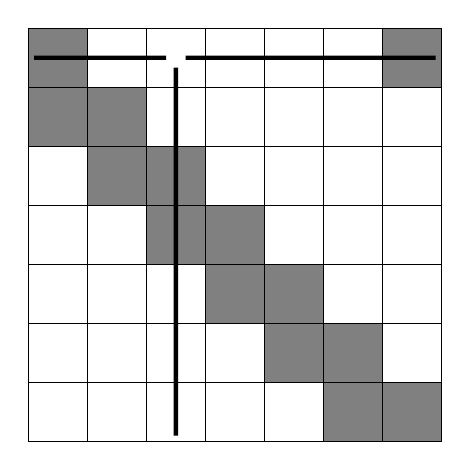
\begin{tikzpicture}[scale = 0.75]
    \foreach \i in {0,...,6} { \fill[gray] (\i, 6 - \i) rectangle (\i + 1, 7 - \i); }
    \foreach \i in {1,...,6} { \fill[gray] (\i-1, 6 - \i) rectangle (\i, 7 - \i); }
    \fill[gray] (6, 6) rectangle (7, 7);
    \draw (0,0) grid (7,7);
    \node (R) at (2.5, 6.5) {\huge\symrook};
    \draw[ultra thick]
      (0.1,6.5) -- (R) -- (6.9,6.5)
      (R) -- (2.5,0.1)
    ;
  \end{tikzpicture}
  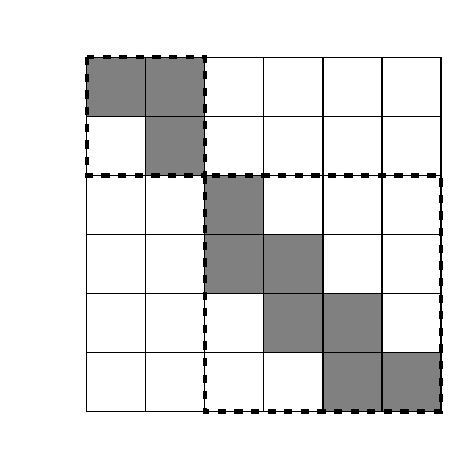
\begin{tikzpicture}[scale = 0.75]
    \path (0,-0.5) -- (0,6.5); % vertically center.
    \foreach \i/\j in {1/5, 2/5, 2/4, 3/3, 3/2, 4/2, 4/1, 5/1, 5/0, 6/0} { \fill[gray] (\i, \j) rectangle (\i + 1, \j + 1); }
    \draw[ultra thick, dashed] (1,6) rectangle (3,4) rectangle (7,0);
    \draw (1,0) grid (7,6);
  \end{tikzpicture}
  \caption{
    The first chessboard shows a placement of a rook at position $3$,
    the second shows the remaining squares, and the third shows a permutation
    of the rows to put the board into a block-diagonal form.
  }
  \label{fig:mengage}
\end{figure}
